\section{Complete Sensitivity Data}
\label{chapter:S2}

% block-id: S2.geometry.heading
\hypertarget{S2.geometry.heading}{}
\subsection{Geometry sampling and discrete transposition}

% block-id: S2.geometry.p1
\hypertarget{S2.geometry.p1}{}
Fig.~\ref{fig:geometry_comparison} shows straight, single-level, traditional multilevel and cross-layer centerlines. The geometry records preserve strand identity, periodicity, clearance, curvature, actual arc length and copper volume. Axial sampling at 400, 800 and 1600 points and 60 checks support sampling consistency for these quantities. The illustrated 24-strand structure with a copper diameter of 0.100 mm has a nominal copper area of approximately 0.1885 mm² and demonstrates geometry construction. A structure meeting the minimum 5 mm² copper area requires separate construction and verification. Three-dimensional views reveal spatial paths; the corresponding field-circuit model evaluates electromagnetic performance.

% block-id: S2.figure.geometry_comparison
\hypertarget{S2.figure.geometry_comparison}{}
\begin{figure*}[!htbp]
\centering
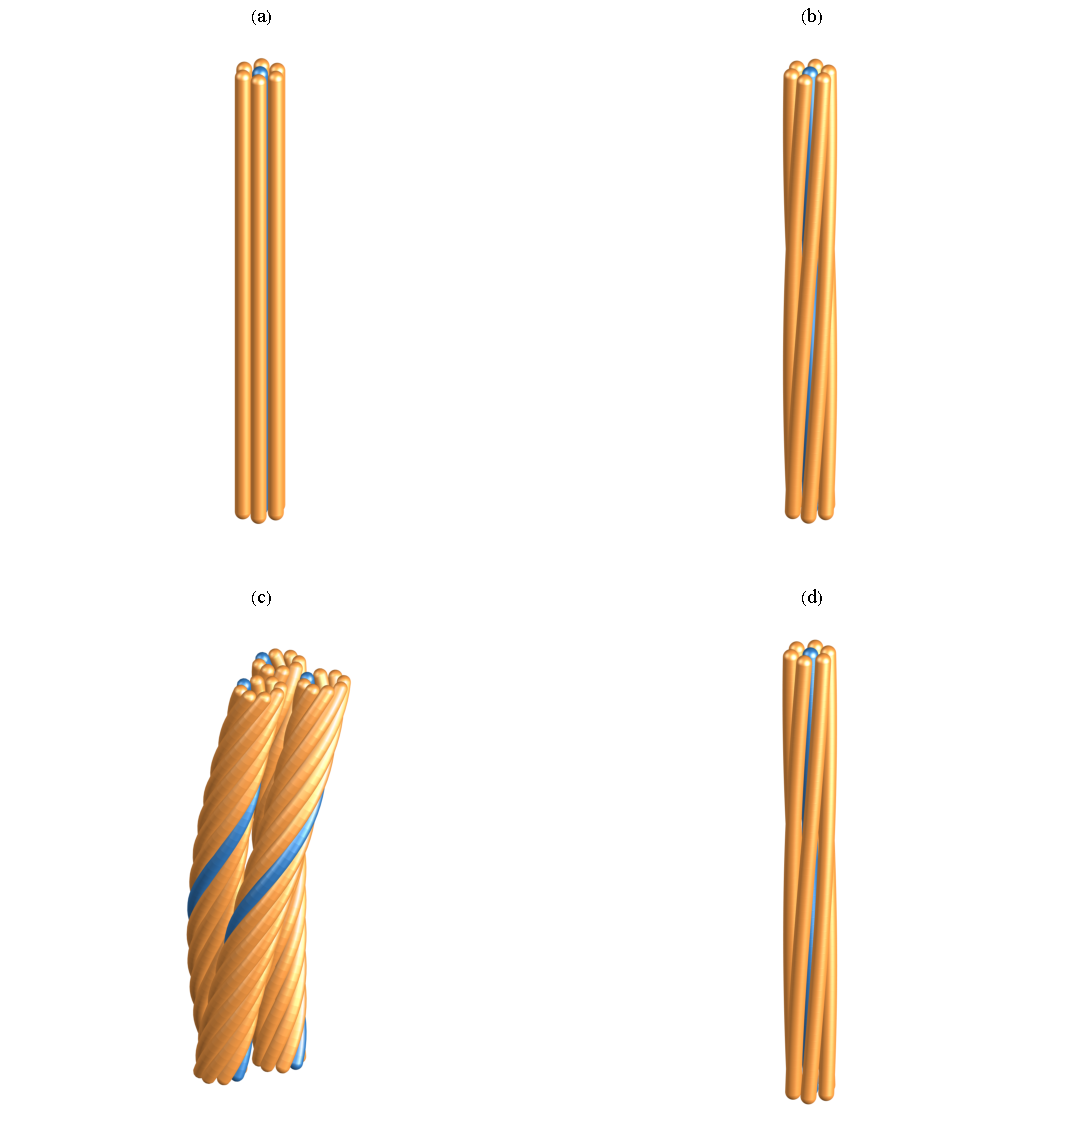
\includegraphics[width=\linewidth,height=.72\textheight,keepaspectratio]{../../assets/en/geometry_comparison.pdf}
\caption{Three-dimensional strand centerline structures. Panels show straight, single-level, local multilevel, and cross-layer structures.}
\label{fig:geometry_comparison}
\end{figure*}

% block-id: S2.geometry.p2
\hypertarget{S2.geometry.p2}{}
The current DTM/iDTM demonstration uses the additive discrete blocks in \eqref{eq:E06}. For the same weighted impedance blocks, their sum is invariant to ordering; this implementation therefore checks identity mappings and circuit accumulation of the specified blocks. Comparing actual transposition paths additionally requires longitudinal position changes, noncommuting relationships between levels, local fields, and terminal conditions. These assumptions determine comparability with the literature \cite{P01,N01}.

% block-id: S2.rt0.heading
\hypertarget{S2.rt0.heading}{}
\subsection{RT0 cuboid under an imposed field}

% block-id: S2.rt0.p1
\hypertarget{S2.rt0.p1}{}
The case is a homogeneous copper cuboid of 1×1×2 mm at 200 kHz, with imposed Bz=1 mT RMS and zero net transport. Three-component current is represented by face-flux degrees of freedom, with separate continuity, port-constraint, and imposed-field power checks. At quadrature q=14, meshes of 8192, 16000, and 27648 cells give losses of 0.927463, 0.933539, and 0.936927 mW. Consecutive refinement changes are 0.655090\% and 0.362916\%, below the 1\% target. Increasing the finest case to q=18 changes loss and complex face flux relatively by 1.55×10⁻⁸ and 1.39×10⁻⁸, respectively, below the 0.1\% quadrature target; see Fig.~\ref{fig:rt0_spatial}.

% block-id: S2.figure.rt0_spatial
\hypertarget{S2.figure.rt0_spatial}{}
\begin{figure}[!htbp]
\centering
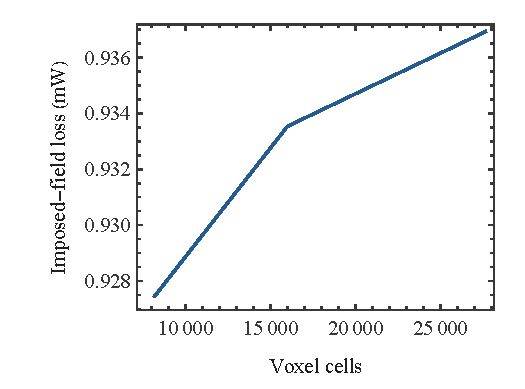
\includegraphics[width=\linewidth,height=.72\textheight,keepaspectratio]{../../assets/en/rt0_spatial.pdf}
\caption{RT0 spatial and integration comparisons. The 1×1×2 mm copper cuboid is excited at 200 kHz by a 1 mT RMS field with zero net transport. The q14 spatial sequence and final q18 comparison use the same imposed-field condition.}
\label{fig:rt0_spatial}
\end{figure}

% block-id: S2.rt0.p2
\hypertarget{S2.rt0.p2}{}
Sections and vectors in Fig.~\ref{fig:rt0_sections} and Fig.~\ref{fig:rt0_vectors} are reconstructed from saved face fluxes. Cell-center current is obtained by averaging opposite-face fluxes and dividing by face area. Cell-average loss density uses the full local RT0 overlap integral and therefore includes within-cell variation. Arrows show the real current at zero phase with one common length scale; color represents the complex RMS norm. Section locations and vector samples follow the figure annotations, while volume integration uses all cells.

% block-id: S2.figure.rt0_sections
\hypertarget{S2.figure.rt0_sections}{}
\begin{figure*}[!htbp]
\centering
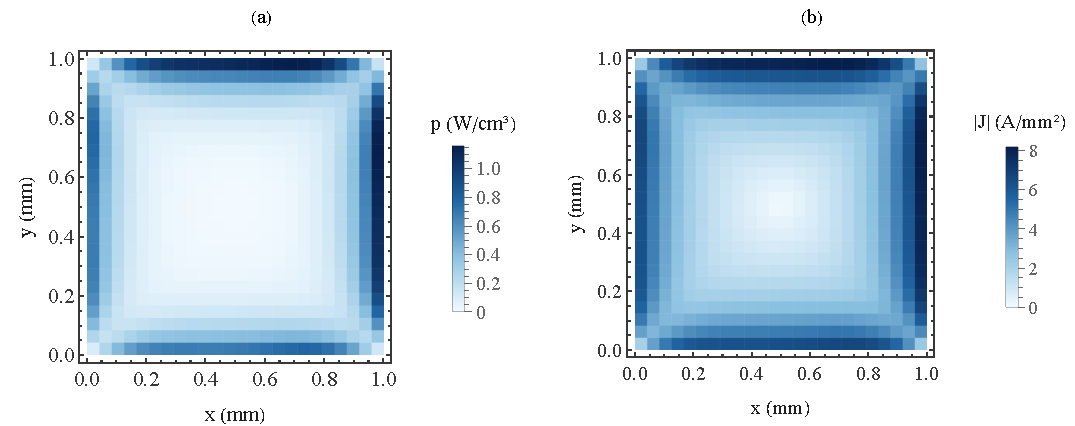
\includegraphics[width=\linewidth,height=.72\textheight,keepaspectratio]{../../assets/en/rt0_sections.pdf}
\caption{RT0 imposed-field current and loss sections. The 1×1×2 mm copper cuboid is excited at 200 kHz by a 1 mT RMS field with zero net transport. (a) Cell-average loss density; (b) complex RMS current norm.}
\label{fig:rt0_sections}
\end{figure*}

% block-id: S2.figure.rt0_vectors
\hypertarget{S2.figure.rt0_vectors}{}
\begin{figure}[!htbp]
\centering
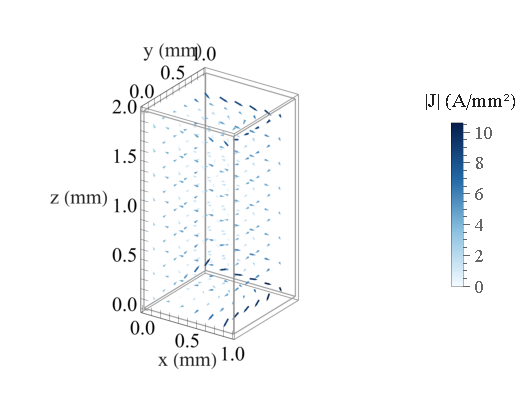
\includegraphics[width=\linewidth,height=.72\textheight,keepaspectratio]{../../assets/en/rt0_vectors.pdf}
\caption{RT0 reconstructed three-dimensional current vectors. The 1×1×2 mm copper cuboid is excited at 200 kHz by a 1 mT RMS field with zero net transport. Arrows show the real part at a fixed phase; color represents the complex RMS norm.}
\label{fig:rt0_vectors}
\end{figure}

% block-id: S2.rt0.p3
\hypertarget{S2.rt0.p3}{}
Each mesh records 35 GMRES iterations and meets the 10⁻¹¹ true-residual target. Spatial and quadrature comparisons jointly support the fixed-cuboid imposed-field result. Applicability has yet to extend to curved Litz masks, independently validated boundary fluxes, and actual transport terminals. The original q=18 summary's missing metrics and failure status, CSV-based postprocessing acceptance, and resource records for dense and matrix-free implementations are retained separately to preserve the relationship between solution and interpretation.

% block-id: S2.aphi.heading
\hypertarget{S2.aphi.heading}{}
\subsection{A–φ cylinder calibration and field–potential diagnostics}

% block-id: S2.aphi.p1
\hypertarget{S2.aphi.p1}{}
The A–φ model recovers current using \eqref{eq:E07} from saved A and actual gradients of φ. The three cylinder meshes contain 1683, 3672, and 9108 nodes; results appear in Fig.~\ref{fig:aphi_gates}. Radial J calibration meets its target on the finest mesh, while φ and gauge residuals fail on all three; the two coarser meshes also fail the J target. Manufactured-solution checks support correspondence between the tested equations and implementation, while physical cylinder calibration reveals field–potential consistency questions requiring further research.

% block-id: S2.equation.E07
\hypertarget{S2.equation.E07}{}
\hypertarget{E07}{}\begin{equation}\mathbf J=-\sigma\left(j\omega\mathbf A+\nabla\phi\right)\tag{9}\label{eq:E07}\end{equation}

% block-id: S2.figure.aphi_gates
\hypertarget{S2.figure.aphi_gates}{}
\begin{figure}[!htbp]
\centering
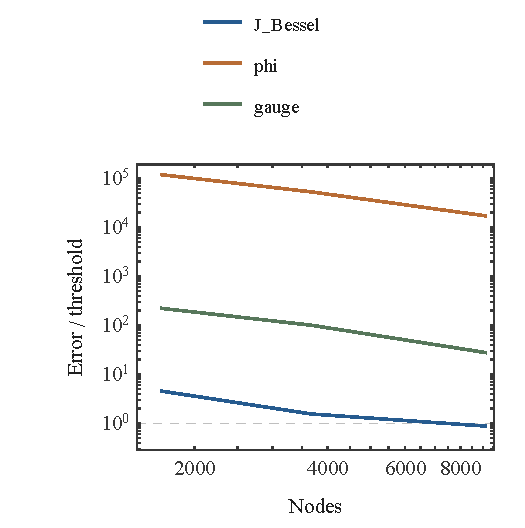
\includegraphics[width=\linewidth,height=.72\textheight,keepaspectratio]{../../assets/en/aphi_gates.pdf}
\caption{A–φ cylinder calibration metrics. Three grids and their metric targets are shown separately.}
\label{fig:aphi_gates}
\end{figure}

% block-id: S2.aphi.p2
\hypertarget{S2.aphi.p2}{}
Fig.~\ref{fig:aphi_preserved} uses 128 explicitly identified nodal samples to display A, φ, J and the actual φ gradient at those locations. The reproduction materials retain boundary, scaling, derivative and postprocessing diagnostics, together with failure causes for direct factorization, out-of-core and iterative routes. These records help distinguish implementation problems from discretization errors. The current cylinder results have not passed physical acceptance.

% block-id: S2.figure.aphi_preserved
\hypertarget{S2.figure.aphi_preserved}{}
\begin{figure*}[!htbp]
\centering
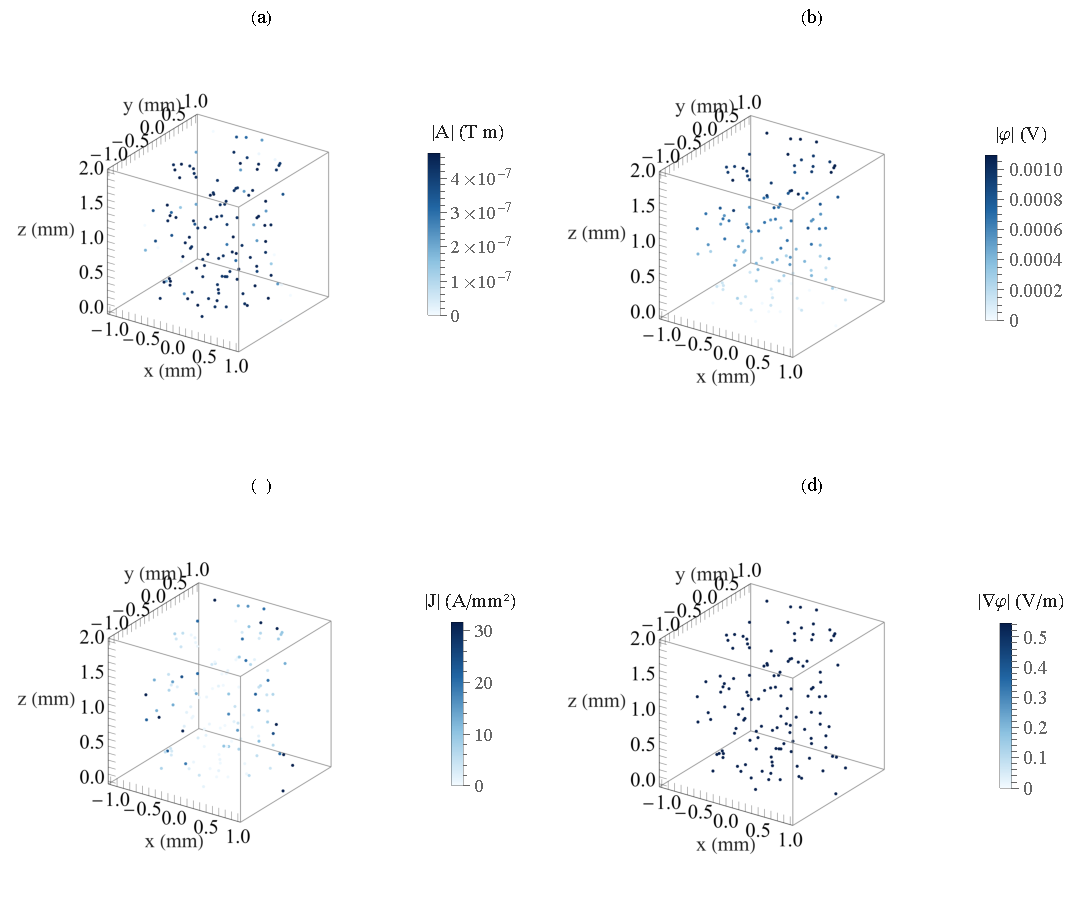
\includegraphics[width=\linewidth,height=.72\textheight,keepaspectratio]{../../assets/en/aphi_preserved.pdf}
\caption{Preserved A–φ field samples. Panels show A, φ, J, and the actual gradient of φ.}
\label{fig:aphi_preserved}
\end{figure*}

% block-id: S2.ansys.heading
\hypertarget{S2.ansys.heading}{}
\subsection{Ansys port validation and capacity}

% block-id: S2.ansys.p1
\hypertarget{S2.ansys.p1}{}
The historical two-dimensional seven-strand port test uses 704 elements, two voltage basis solutions, and a third actual ±20 A field solution. Common terminal voltage, complex strand currents, and independent power establish field–circuit consistency on that mesh; current results appear in Fig.~\ref{fig:ansys_seven_current}. Validation concerns one mesh. Subsequent fixed-mesh and precision attempts have not completed the required three-level checks, and the native three-dimensional J-expression probe has not produced an acceptable physical solution.

% block-id: S2.figure.ansys_seven_current
\hypertarget{S2.figure.ansys_seven_current}{}
\begin{figure}[!htbp]
\centering
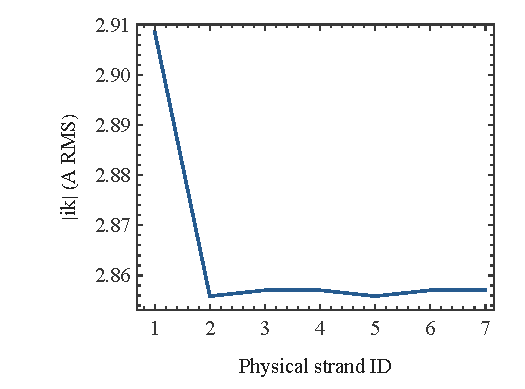
\includegraphics[width=\linewidth,height=.72\textheight,keepaspectratio]{../../assets/en/ansys_seven_current.pdf}
\caption{Ansys seven-strand two-dimensional complex currents. The valid 704-cell port short test provides strand magnitudes and phases.}
\label{fig:ansys_seven_current}
\end{figure}

% block-id: S2.ansys.p2
\hypertarget{S2.ansys.p2}{}
Fig.~\ref{fig:ansys_limits} summarizes the verified Ansys Student v252 limits: up to 2000 triangles in two dimensions, 64000 volume elements and 8000 surface elements in three dimensions, and at most four processor cores. Interface capability, licensed model size and numerical accuracy separately constrain executable validation. Actual terminations, curved STL geometry and large bundles with sufficient copper area require licensing and mesh capacity appropriate to the target geometry, followed by sensitivity and power-balance checks.

% block-id: S2.figure.ansys_limits
\hypertarget{S2.figure.ansys_limits}{}
\begin{figure}[!htbp]
\centering
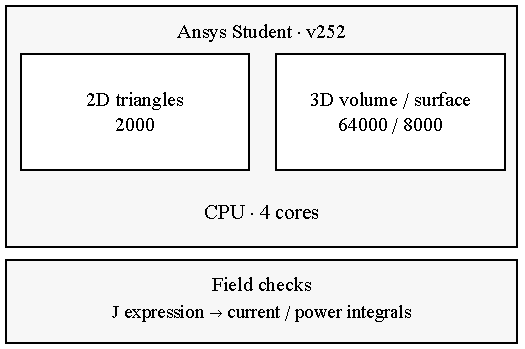
\includegraphics[width=\linewidth,height=.72\textheight,keepaspectratio]{../../assets/en/ansys_limits.pdf}
\caption{Ansys Student capacity and interface diagnostics. License capacity and field-check entry points for Ansys Student v252: 2000 triangles in two dimensions, 64000 volume and 8000 surface elements in three dimensions, and up to four compute cores. Capacity information is retained from rc.1 records; figure sources were checked on 2026-10-15.}
\label{fig:ansys_limits}
\end{figure}

% block-id: S2.tables
\hypertarget{S2.tables}{}
\begin{table*}[!htbp]
\centering
\caption{Round-wire two-dimensional calibration}
\label{tab:S2.tables-0}
\begingroup\footnotesize
\begin{tabularx}{\textwidth}{>{\raggedright\arraybackslash}X>{\raggedright\arraybackslash}X>{\raggedright\arraybackslash}X>{\raggedright\arraybackslash}X}
\toprule
Nodes & h/a & Rac (mΩ/m) & Relative resistance error\\
\midrule
353 & 0.24 & 20.1572 & 0.00704525\\
1389 & 0.12 & 20.0208 & 0.000230269\\
5573 & 0.06 & 20.0162 & 1.79233e-06\\
\bottomrule
\end{tabularx}
\endgroup
\end{table*}
\begin{table*}[!htbp]
\centering
\caption{Longitudinal PEEC length sensitivity}
\label{tab:S2.tables-1}
\begingroup\footnotesize
\begin{tabularx}{\textwidth}{>{\raggedright\arraybackslash}X>{\raggedright\arraybackslash}X>{\raggedright\arraybackslash}X>{\raggedright\arraybackslash}X}
\toprule
Degrees of freedom & Length (m) & Rac (mΩ/axial m) & Rac/Rdc\\
\midrule
1264 & 0.16 & 19.8992 & 3.64713\\
1264 & 0.32 & 19.9586 & 3.65802\\
1264 & 0.64 & 19.9885 & 3.66349\\
5024 & 0.32 & 19.983 & 3.63931\\
5024 & 0.64 & 20.0127 & 3.64472\\
\bottomrule
\end{tabularx}
\endgroup
\end{table*}
\begin{table*}[!htbp]
\centering
\caption{RT0 imposed-field loss and quadrature order}
\label{tab:S2.tables-2}
\begingroup\footnotesize
\begin{tabularx}{\textwidth}{>{\raggedright\arraybackslash}X>{\raggedright\arraybackslash}X>{\raggedright\arraybackslash}X}
\toprule
Cells & Quadrature order & Loss (mW)\\
\midrule
8192 & 14 & 0.927463\\
16000 & 14 & 0.933539\\
27648 & 14 & 0.936927\\
27648 & 18 & 0.936927\\
\bottomrule
\end{tabularx}
\endgroup
\end{table*}
\begin{table*}[!htbp]
\centering
\caption{CPU/GPU comparison for the same model}
\label{tab:S2.tables-3}
\begingroup\footnotesize
\begin{tabularx}{\textwidth}{>{\raggedright\arraybackslash}X>{\raggedright\arraybackslash}X>{\raggedright\arraybackslash}X}
\toprule
Degrees of freedom & Relative inductance difference & Relative current difference\\
\midrule
1264 & 7.07572e-16 & 3.28174e-14\\
5024 & 7.48149e-16 & 7.78082e-14\\
\bottomrule
\end{tabularx}
\endgroup
\end{table*}
\begin{table*}[!htbp]
\centering
\caption{PEEC sensitivity plot indices and values}
\label{tab:S2.tables-4}
\begingroup\footnotesize
\begin{tabularx}{\textwidth}{>{\raggedright\arraybackslash}X>{\raggedright\arraybackslash}X>{\raggedright\arraybackslash}X}
\toprule
Plot index & Single-factor comparison & Plotted relative change (\%)\\
\midrule
1 & length\_\allowbreak 016\_\allowbreak 032 & 0.29864\\
2 & length\_\allowbreak 032\_\allowbreak 064 & 0.149482\\
3 & fine\_\allowbreak length\_\allowbreak 032\_\allowbreak 064 & 0.14873\\
4 & mutual\_\allowbreak q4\_\allowbreak to6 & 0.001597\\
5 & mutual\_\allowbreak q6\_\allowbreak to8 & 0.000588978\\
6 & fine\_\allowbreak mutual\_\allowbreak q4\_\allowbreak to6 & 0.000462112\\
7 & fine\_\allowbreak mutual\_\allowbreak q6\_\allowbreak to8 & 0.000169935\\
8 & self\_\allowbreak 10p8\_\allowbreak to12p10 & 7.09596e-09\\
9 & fine\_\allowbreak self\_\allowbreak 10p8\_\allowbreak to12p10 & 1.84501e-09\\
10 & spatial\_\allowbreak l032 & 0.122127\\
11 & spatial\_\allowbreak l064 & 0.121376\\
\bottomrule
\end{tabularx}
\endgroup
\end{table*}

% block-id: S2.ansys.rc2
\hypertarget{S2.ansys.rc2}{}
The rc.2 records additionally complete two-dimensional Maxwell construction, solution, and project readback through PyAEDT-MCP, with task cancellation and linked restart records. A seven-strand straight-bundle comparison with Wolfram aligns cross-section, material, frequency, return, and total-current constraints. Relative complex-current L2 and bundle Rac differences are 0.0106814\% and 0.00132823\%, respectively. The implementations use independent meshes, Maxwell performs one adaptive pass, and spatial and boundary convergence remain to be checked. This success establishes the corresponding two-dimensional port workflow; three-dimensional interfaces and transposed structures with sufficient copper require their own field solutions and acceptance. \cite{PYAEDTMCP,PYAEDT}

% block-id: S2.method.sources
\hypertarget{S2.method.sources}{}
The RT0 face-flux representation follows the lowest-order mixed finite-element space. Nonsymmetric discrete systems use GMRES with true-residual checks. The field–potential implementation and quasistatic magnetic-field documentation inform diagnosis of A–φ boundaries and gauge treatment. \cite{RT1977,GMRES1986,FEMDOC}
